\chapter{Referencial Teórico}
\label{cap:ref-teorico}

\section{\gls{NPM}}
\label{ref-teo:npm}
O \gls{NPM} é um projeto \textit{open-source} de gerenciamento de pacotes para o \textit{Node.js}. Lançado em 2009, seu principal objetivo é facilitar o compartilhamento de códigos escrito, principalmente, em \textit{Javascript}. Intitulada com o mesmo nome, a \gls{NPM} \textit{Inc} é um repositório online de publicação e compartilhamento de projetos. Atualmente, o \gls{NPM} ocupa a posição de maior repositório para uma dada linguagem com mais de 1 milhão de projetos\footnote{http://www.modulecounts.com/}, enquanto que o segundo maior repositório -- \textit{Maven} -- contém pouco mais de 200 mil  projetos. O ecossistema \gls{NPM} é caracterizado por \citeonline{teorical_reference:npm} por abranger diferentes plataformas de \textit{software}, distribuído em múltiplos sistemas e gerenciado por várias entidades.

O \gls{NPM} permite que, com apenas um simples comando, o usuário realize o download, publique, instale, desinstale pacotes diretamente do repositório do \gls{NPM} entre outras tarefas. A facilidade proporcionada pelo \gls{NPM} corrobora para a grande popularidade do \textit{Javascript} e para que o compartilhamento de biblioteca seja largamente utilizado, uma vez que 97\% dos aplicativos \textit{web} são oriundos do \textit{NPM}\footnote{https://blog.npmjs.org/post/180868064080/this-year-in-javascript-2018-in-review-and-npms}.
%In fact, 97\% of the code in a modern web application comes from npm

\section{Node.js}
\label{ref-teo:node}
O \textit{Node.js} é um projeto \textit{open-source} implementado em \textit{C++} sobre a \textit{engine Javascript V8} do \textit{Google}, que é um compilador \textit{Javascript} para \textit{web}. O \textit{Node.js} foi criado com o objetivo de estender o código \textit{Javascript} para além das páginas \textit{web}: agora o código \textit{Javascript} pode ser executado nos servidores. Com o \textit{Javascript} executando no \textit{front-end} e no \textit{back-end} não se faz necessário que os desenvolvedores saibam duas linguagens de programação diferentes, pois o \textit{Javascript} pode ser utilizado em ambos os contextos. A dualidade de utilização do \textit{Javascript} permitida pelo \textit{Node.js} foi um dos principais fatores que levou à grande popularidade do \textit{Javascript}, uma vez que o \textit{Node.js} é o \textit{framework} mais utilizado atualmente, de acordo com o \textit{Stack Overflow}\footnote{https://insights.stackoverflow.com/survey/2019\#technology-_-other-frameworks-libraries-and-tools}.

\section{\gls{SemVer}}
\label{ref-teo:semver}
O \gls{SemVer}\footnote{https://semver.org} é um padrão para versionamento de \textit{releases} de um projeto a partir do tipo de alteração introduzida na \textit{release}. Com o \gls{SemVer} é possível evoluir um projeto sempre mantendo a compatibilidade com versões anteriores através de um \textit{range de versões} na qual está especificada uma determinada versão. O padrão \gls{SemVer} é largamente utilizada no desenvolvimento de projetos. As regras do \gls{SemVer} foram idealizadas por Tom Preston-Werner -- criador do \textit{GitHub} -- que incentiva todos os desenvolvedores à utilizarem este padrão, uma vez que as regras são baseadas em práticas comuns já utilizadas em projetos \cite{teorical_reference:semver}.

O esquema de versionamento, basicamente, é uma \textit{string} que possui três dígitos: \textit{major.minor.path}. Os dígitos do \gls{SemVer} devem ser incrementados de acordo com o tipo de alteração que a \textit{release} do projeto está introduzindo. O número \textit{major} deve ser incrementado quando uma \textit{release} introduz \textit{breaking changes}; o \textit{minor}, quando é adicionada melhorias/novas funcionalidades que mantenham a compatibilidade com as \textit{releases} anteriores; e o \textit{path}, quando a \textit{release} contém correção de \textit{bugs}. Com a padronização do \gls{SemVer} é possível que os desenvolvedores introduzem \textit{breaking changes} sem que essas afetem os clientes, uma vez que, por meio da \textit{string} de versionamento, eles não receberão a \textit{release} com \textit{breaking changes}.

O \gls{NPM} utiliza o padrão \gls{SemVer} no arquivo \textit{package.json} -- arquivo de configuração do projeto que contém todas as suas dependências e suas respectivas versões. Ao executar o comando \textit{npm install express --save}, para instalar a dependência \textit{express}\footnote{https://www.npmjs.com/package/express} por exemplo, o \gls{NPM} -- além de descarregar essa dependência -- irá salvar no \textit{package.json} o nome dessa dependência com sua versão atual em modo \textit{range}, de acordo com a Figura \ref{fig:dep_express}.

\begin{figure}
    \centering
    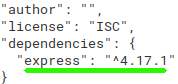
\includegraphics{figuras/dependencies_express.png}
    \caption{Modo como o \gls{NPM} salva no \textit{package.json} a versão de uma dependência}
    \label{fig:dep_express}
\end{figure}{}

Com a informação da versão da dependência no \textit{package.json}, o cliente não precisa se preocupar com as novas atualizações de sua dependência, uma vez que o \gls{NPM}, ao instalar novamente as dependências, sempre irá descarregar a \textit{release} mais recente da dependência que não contenha uma \textit{breaking change}, ou seja, a última \textit{release} disponível para a mesma versão \textit{major} -- desde que a \textit{string} de versionamento seja salva em modo \textit{range} (\textasciicircum).

\section{Checkout}
\label{ref-teo:checkout}
\textit{Checkout} é uma palavra que pode ter vários sentidos, tanto em um contexto geral como na área científica da computação. Neste artigo, \textit{checkout} se refere ao efeito da execução do comando \textit{git checkout} em um repositório clonado do \textit{GitHub}. Este comando realiza diversas alterações na \textit{working tree} do repositório -- lista de arquivos atuais. Dentre as alterações, podem ser citadas a criação e a alteração das \textit{branchs} do repositório, atualização do estado de um determinado arquivo para o seu estado no \textit{HEAD} do repositório, alteração da \textit{working tree} para o estado de um determinado \textit{commit} entre outras ações\footnote{https://git-scm.com/docs/git-checkout}. Entretanto, o que se refere ao \textit{checkout} neste artigo é a alteração da \textit{working tree} para um determinado estado de um repositório em um intervalo de tempo definido por dois \textit{timestamp} -- os \textit{timestamp} do intervalo entre duas versões.

Um repositório clonado do \textit{GitHub} contém os arquivos no seu estado mais atual. Entretanto, faz-se necessário restaurar os arquivos ao estado de uma \textit{release} específica, e isso é realizado através do comando \textit{git checkout}. Os parâmetros passados à este comando são os \textit{timestamp} das \textit{releases}, que são recuperadas da \textit{API} do \gls{NPM}\footnote{http://registry.npmjs.org/} para cada \textit{release} de um determinado pacote. Assim, é possível restaurar a \textit{working tree} para o estado do qual a determinada \textit{release} se encontrava. Com isto, todos os arquivos serão os mesmos.

\section{Breaking Change}
\label{ref-teo:breaking_change}
Uma \textit{break change} é uma alteração no pacote provedor que resulta em erros inesperados nos pacotes clientes, uma vez que versões prévias do pacote provedor executava normalmente \cite{teorical_reference:semver}. O conceito de \textit{breaking changes} não se refere exclusivamente à \textit{erros} causados pelos provedores, mas sim à mudanças nos pacotes. Durante o desenvolvimento de \textit{software}, esses precisam introduzir \textit{breaking changes}, pois quando só há \textit{releases} compatíveis com versões anteriores o pacote perde muitas oportunidades de evolução \cite{teorical_reference:bc_2}. Entretanto, a \textit{breaking change} pode ser introduzida em uma \textit{release} intencionalmente -- quando é atualizada a versão \textit{major} da \textit{release} --, mas também pode ser introduzida impremeditadamente -- quando é atualizada sua versão no \textit{minor} ou \textit{path} da \textit{release}. Sempre que \textit{breaking changes} são introduzidas inesperadamente, há grandes chances de ocorrer falhas no código cliente.

As \textit{breaking changes} são mais expressivas em linguagem fortemente tipadas, tais como \textit{.NET} e \textit{Java}, tanto que há ferramentas para detectar \textit{breaking changes} nestas linguagens. Já nas linguagens dinâmicas, como a linguagem \textit{Javascript}, as \textit{breaking changes} surgem com menos frequências e nem possuem ferramentas para detectar as \textit{breaking changes} \cite{teorical_reference:bc_1}. Como exemplo da dinâmica da linguagem \textit{Javascript}, considere a Figura \ref{fig:non-bc-async}.

\begin{figure}
    \centering
    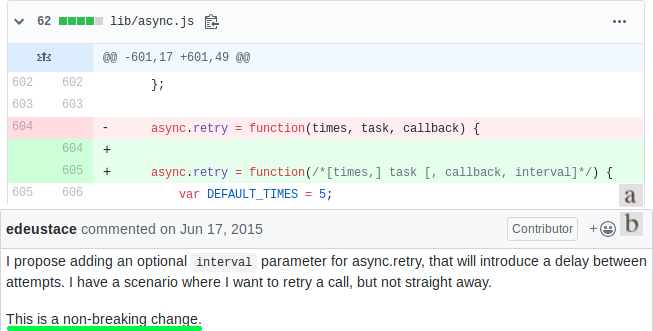
\includegraphics[scale=0.6]{figuras/non-bc-async.png}
    \caption{(a) alteração \textit{non-breaking change} entre duas \textit{releases minor}; (b) comentário do desenvolvedor afirmando que sua alteração não é uma \textit{breaking change}}
    \label{fig:non-bc-async}
\end{figure}{}

Na Figura \ref{fig:non-bc-async} (a) há uma alteração em uma das \gls{API} do pacote \textit{async} entre as \textit{releases 1.2.1-1.3}. Nesta alteração, houve a remoção da lista de parâmetros da função \textit{async.retry}. Em uma linguagem tipada, como o \textit{Java}, a alteração da lista de parâmetros é uma \textit{breaking change} e foi constatado como a terceira maior causa de \textit{breaking changes} em bibliotecas hospedados no \textit{Maven} -- repositório de bibliotecas em \textit{Java} -- em um estudo realizado por \citeonline{teorical_reference:semver}.

Entretanto, em linguagens dinâmicas como a linguagem \textit{Javascript}, a alteração da lista de parâmetros não é considerada uma \textit{breaking change}, pois o desenvolvedor que realizou o \textit{pull-request}\footnote{https://github.com/caolan/async/pull/793} da \ref{fig:non-bc-async} (a) comentou que esta alteração não é uma \textit{breaking change}, conforme a da Figura \ref{fig:non-bc-async} (b). Realmente, não é uma \textit{breaking change}, uma vez que uma chamada para a função \textit{async.retry}, seja na \textit{release 1.2.1} ou na \textit{release 1.3}, o código executa normalmente. Mesmo com esta alteração, um código irá executar em qualquer versão, uma vez que o \textit{node.js} insere os argumentos da chamada de função em um \textit{Array}, o que permite que qualquer função possa ser executada com qualquer número de argumentos\footnote{https://developer.mozilla.org/en-US/docs/Web/JavaScript/Reference/Functions/arguments}. Mesmo com a dinâmica da linguagem \textit{Javascript}, essa possui sim \textit{breaking changes}.

\section{Pacote, \textit{Release} e Versão}
\label{ref-teo:release}
Neste artigo, a palavra \textit{pacote} refere-se a um \textit{software} hospedado no \gls{NPM}. Este \textit{software} contém seu nome, sua marca, seus arquivos, suas versões etc. e tudo mais que a ele pertence. Por exemplo, quando nos referimos ao pacote \textit{mocha}, nos referimos à ideia genérica deste pacote, sem levar em consideração uma versão específica ou seu estado em algum instante, mas sim, apenas ao pacote como um todo.

Já a palavra \textit{release} designa o estado de um pacote em um determinado instante. Ou seja, uma \textit{release} significa uma versão específica deste pacote, isto é, um conjunto de arquivos distintos das demais \textit{releases}. Por exemplo, o primeiro publicação de um pacote será sua primeira \textit{release}; a segunda, sua segunda \textit{release}; a terceira, sua terceira \textit{release} e assim por diante\footnote{https://www.computerhope.com/jargon/r/release.htm}.

Por fim, o termo \textit{versão} é utilizado para especificar e distinguir um determinado estado de uma \textit{release}. Uma \textit{versão} é uma \textit{string} no padrão \gls{SemVer} que identifica unicamente uma determinada \textit{release} e é utilizada pelo \gls{NPM} no arquivo \textit{package.json} para evitar conflitos entre duas \textit{releases}.

\section{Dependência Direta e Indireta}
\label{ref-teo:dep_di_ind}
